%! TeX program = lualatex
\documentclass[12pt, fleqn]{extarticle}
\usepackage[english,russian]{babel}
\usepackage{fontspec}
\usepackage{graphicx}
\usepackage{indentfirst}
\usepackage{caption}
\usepackage{wrapfig}
\usepackage{amsmath}
\usepackage{hyperref}
% \usepackage{geometry}
% \usepackage{emoji}
% \usepackage{amsmath}
% \usepackage{xcolor, cancel}
% \usepackage{stackengine}
% \usepackage{ulem}
% \usepackage{amsthm}
% \usepackage{tikz}
% \usepackage{multicol}
% \usepackage{pgfplots}
% \usepackage{ragged2e}
% \usepackage{xifthen}
% \usepackage{amssymb}
% \usepackage{unicode-math}
% \usepackage{textcomp}

\setmainfont{PT Serif}

\usepackage[%
    left=1.25in,%
    right=1.25in,%
    top=1.1in,%
    bottom=1.1in,%
]{geometry}%

\hypersetup{
    colorlinks=true,
    linkcolor=black,
    filecolor=magenta,
    urlcolor=cyan,
    pdftitle={Ответы на билеты по математике 2021},
    pdfpagemode=FullScreen,
}

\captionsetup[figure]{labelformat=empty, labelsep=none}
\graphicspath{ {./images/} }

\begin{document}

\section*{Быстрое перемещение}

Для перемещения \textbf{нажмите} на название требуемого раздела:
\begin{enumerate}
    \item \hyperref[sec:det]{Свойства определителей}
    \item \hyperref[sec:line_1]{Прямая на плоскости: уравнение через две точки, каноническое, параметрическое}
    \item \hyperref[sec:parabola]{Парабола. Определение, вывод уравнения, характеристики}
\end{enumerate}

\newpage

\section*{Свойства определителей}\label{sec:det}

1. Определитель транспонированной матрицы равен определителю исходной матрицы: \(\det A^T = \det A\)

2. Умножение всех элементов строки или столбца определителя на некоторое число \lambda равносильно умножееию определителя на это число:
\begin{align*}
     &  &
    \begin{vmatrix}
        a_{11}         & a_{12}         & \dots a_{1j}         & \dots & a_{1n}         \\
        a_{21}         & a_{22}         & \dots a_{2j}         & \dots & a_{2n}         \\
        \dots          & \dots          & \dots                & \dots & \dots          \\
        \lambda a_{i1} & \lambda a_{i2} & \dots \lambda a_{ij} & \dots & \lambda a_{in} \\
        \dots          & \dots          & \dots                & \dots & \dots          \\
        a_{m1}         & a_{m2}         & \dots a_{mj}         & \dots & a_{mn}         \\
    \end{vmatrix}
    =
    \lambda \cdot
    \begin{vmatrix}
        a_{11} & a_{12} & \dots a_{1j} & \dots & a_{1n} \\
        a_{21} & a_{22} & \dots a_{2j} & \dots & a_{2n} \\
        \dots  & \dots  & \dots        & \dots & \dots  \\
        a_{i1} & a_{i2} & \dots a_{ij} & \dots & a_{in} \\
        \dots  & \dots  & \dots        & \dots & \dots  \\
        a_{m1} & a_{m2} & \dots a_{mj} & \dots & a_{mn} \\
    \end{vmatrix}
\end{align*}

3. Если в определителе переставить местами любые две строки или два столбца, то определитель изменяет свой знак на противоположный:
\begin{align*}
     &  &
    \begin{vmatrix}
        \dots  & \dots  & \dots  & \dots & \dots  \\
        a_{i1} & a_{i2} & a_{i3} & \dots & a_{in} \\
        \dots  & \dots  & \dots  & \dots & \dots  \\
        a_{k1} & a_{k2} & a_{k3} & \dots & a_{kn} \\
        \dots  & \dots  & \dots  & \dots & \dots  \\
    \end{vmatrix}
    =
    -
    \begin{vmatrix}
        \dots  & \dots  & \dots  & \dots & \dots  \\
        a_{k1} & a_{k2} & a_{k3} & \dots & a_{kn} \\
        \dots  & \dots  & \dots  & \dots & \dots  \\
        a_{i1} & a_{i2} & a_{i3} & \dots & a_{in} \\
        \dots  & \dots  & \dots  & \dots & \dots  \\
    \end{vmatrix}
\end{align*}

4. Если матрица содержит нулевую строку (столбец), то определитель этой матрицы равен нулю:
\begin{align*}
     &  &
    \begin{vmatrix}
        \dots  & \dots  & \dots  & \dots & \dots  \\
        a_{i1} & a_{i2} & a_{i3} & \dots & a_{in} \\
        0      & 0      & 0      & \dots & 0      \\
        a_{j1} & a_{j2} & a_{j3} & \dots & a_{jn} \\
        \dots  & \dots  & \dots  & \dots & \dots  \\
    \end{vmatrix}
    = 0
\end{align*}

5. Если две строки (столбца) матрицы равны между собой, то определитель этой матрицы равен нулю:
\begin{align*}
     &  &
    \begin{vmatrix}
        \dots  & \dots  & \dots  & \dots & \dots  \\
        a_{i1} & a_{i2} & a_{i3} & \dots & a_{in} \\
        \dots  & \dots  & \dots  & \dots & \dots  \\
        a_{i1} & a_{i2} & a_{i3} & \dots & a_{in} \\
        \dots  & \dots  & \dots  & \dots & \dots  \\
    \end{vmatrix}
    = 0
\end{align*}

6. Если две строки (столбца) матрицы пропорциональны друг другу, то определитель этой матрицы равен нулю:
\begin{align*}
     &  &
    \begin{vmatrix}
        \dots   & \dots   & \dots   & \dots & \dots   \\
        a_{i1}  & a_{i2}  & a_{i3}  & \dots & a_{in}  \\
        \dots   & \dots   & \dots   & \dots & \dots   \\
        ca_{i1} & ca_{i2} & ca_{i3} & \dots & ca_{in} \\
        \dots   & \dots   & \dots   & \dots & \dots   \\
    \end{vmatrix}
    = 0
\end{align*}

7. Определитель матрицы треугольного вида равен произведению элементов, стоящих на главной диагонали:
\begin{align*}
     &  &
    \begin{vmatrix}
        a_{11} & a_{12} & a_{13} & \dots & a_{1n} \\
        0      & a_{22} & a_{23} & \dots & a_{2n} \\
        0      & 0      & a_{33} & \dots & a_{3n} \\
        \dots  & \dots  & \dots  & \dots & \dots  \\
        0      & 0      & 0      & \dots & a_{mn} \\
    \end{vmatrix}
    = a_{11} \cdot a_{22} \cdot a_{33} \cdot ... \cdot a_{mn}
\end{align*}

8. Если все элементы k-ой строки (столбца) определителя представлены в виде сумм \(a_{kj} + b_{kj}\), то определитель можно представить в виде суммы соответствующих определителей:
\begin{align*}
     &  &
    \begin{vmatrix}
        a_{11}          & a_{12}          & a_{13}          & \dots & a_{1n}          \\
        \dots           & \dots           & \dots           & \dots & \dots           \\
        a_{k1} + b_{k1} & a_{k2} + b_{k2} & a_{k3} + b_{k3} & \dots & a_{kn} + b_{kn} \\
        \dots           & \dots           & \dots           & \dots & \dots           \\
        a_{m1}          & a_{m2}          & a_{m3}          & \dots & a_{mn}          \\
    \end{vmatrix}
    =
    \\
     &  &
    =
    \begin{vmatrix}
        a_{11} & a_{12} & a_{13} & \dots & a_{1n} \\
        \dots  & \dots  & \dots  & \dots & \dots  \\
        a_{k1} & a_{k2} & a_{k3} & \dots & a_{kn} \\
        \dots  & \dots  & \dots  & \dots & \dots  \\
        a_{m1} & a_{m2} & a_{m3} & \dots & a_{mn} \\
    \end{vmatrix}
    +
    \begin{vmatrix}
        a_{11} & a_{12} & a_{13} & \dots & a_{1n} \\
        \dots  & \dots  & \dots  & \dots & \dots  \\
        b_{k1} & b_{k2} & b_{k3} & \dots & b_{kn} \\
        \dots  & \dots  & \dots  & \dots & \dots  \\
        a_{m1} & a_{m2} & a_{m3} & \dots & a_{mn} \\
    \end{vmatrix}
\end{align*}

9. Определитель не изменится, если к элементам любой его строки (или столбца) прибавить соответствующие элементы другой строки (или соответствующего столбца), умноженные на одно и тоже число:
\begin{align*}
     &  &
    \begin{vmatrix}
        \dots  & \dots  & \dots  & \dots & \dots  \\
        a_{i1} & a_{i2} & a_{i3} & \dots & a_{in} \\
        \dots  & \dots  & \dots  & \dots & \dots  \\
        a_{k1} & a_{k2} & a_{k3} & \dots & a_{kn} \\
        \dots  & \dots  & \dots  & \dots & \dots  \\
    \end{vmatrix}
    =
    \begin{vmatrix}
        \dots            & \dots            & \dots            & \dots & \dots            \\
        a_{i1}           & a_{i2}           & a_{i3}           & \dots & a_{in}           \\
        \dots            & \dots            & \dots            & \dots & \dots            \\
        a_{k1} + ca_{i1} & a_{k2} + ca_{i2} & a_{k3} + ca_{i3} & \dots & a_{kn} + ca_{in} \\
        \dots            & \dots            & \dots            & \dots & \dots            \\
    \end{vmatrix}
\end{align*}

10. Пусть A и B – квадратные матрицы одного и того же порядка. Тогда определитель произведения матриц равен произведению определителей:
\begin{align*}
     &  &
    \det (AB) = \det A \cdot \det B
\end{align*}

\newpage

\section*{Прямая на плоскости: уравнение через две точки, каноническое, параметрическое}\label{sec:line_1}

\subsection*{Каноническое уравнение прямой}

Дана прямая \(L\), проходящая через точку \(M_0(x_0;y_0)\), и направляющий вектор \(\overrightarrow{a}(m, n)\) этой прямой.
Пусть \(M(x, y)\) — произвольная точка на искомой прямой \(L\), тогда \(M \in L \iff \overrightarrow{M_0M} || \overrightarrow{a}\).

\begin{center}
    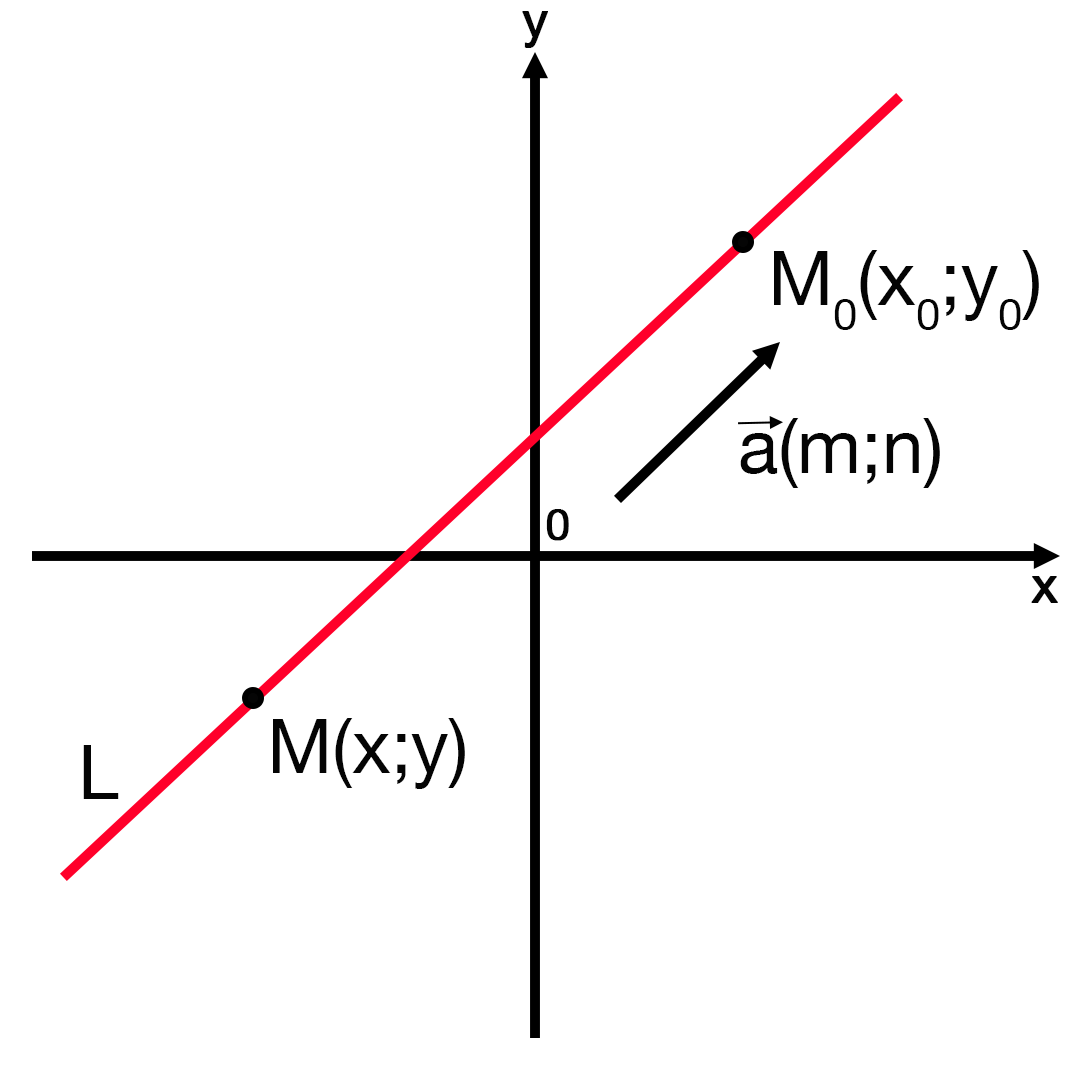
\includegraphics[width=0.5\textwidth]{kanon_line.png}
\end{center}

Условием коллинеарности векторов \(\overrightarrow{M_0M}\) и \(\overrightarrow{a}\) будет:
\(\dfrac{x - x_0}{m} = \dfrac{y - y_0}{n}\), что и является каноническим уравнением прямой.

\subsection*{Уравнение прямой через 2 заданные точки}

Даны две точки \(M_0(x_0;y_0)\) и \(M_1(x_1;y_1)\), лежащие на прямой \(L\).
Из этого следует, что \(\overrightarrow{M_0M_1} = (x_1 - x_0; y_1 - y_0)\) — направляющий вектор прямой \(L\).

Тогда искомое уравнение будет иметь вид: \(\dfrac{x - x_0}{x_1 - x_0} = \dfrac{y - y_0}{y_1 - y_0}\).

\subsection*{Параметрическое уравнение прямой}

Уравнение \(\overrightarrow{M_0M} = \lambda \cdot \overrightarrow{a}\) называют векторно-параметрическим уравнением прямой, где \lambda — некоторое действительное число.

В векторной форме оно имеет вид:
\begin{align*}
     &  &
    \overrightarrow{M_0M} = \lambda \cdot \overrightarrow{a} \iff
    \begin{cases}
        x - x_0 = \lambda \cdot m \\
        y - y_0 = \lambda \cdot n
    \end{cases}
    \iff
    \begin{cases}
        x = x_0 + \lambda \cdot m \\
        y = y_0 + \lambda \cdot n
    \end{cases}
\end{align*}

\section*{Парабола. Определение, вывод уравнения, характеристики}\label{sec:parabola}

\subsection*{Определение}
Парабола — геометрическое место точек на плоскости, равноудалённых от данной прямой \(d\) и данной точки \(F\).
Точка \(F\) не лежит ни на кривой, ни на прямой \(d\).

Точка \(F\) называется \textbf{фокусом}, а прямая \(d\) — \textbf{директрисой параболы}.
Расстояние от фокуса до директрисы называется \textbf{фокальным параметром} параболы и обозначается через \(p\).

\textbf{Эксцентриситет} параболы — это отношение расстояний от произвольной точки на кривой до фокуса и от этой же точки до директрисы.
Эксцентриситет параболы по определению равен 1.

Каноническое уравнение параболы: \(y^2 = 2px\)

\subsection*{Вывод канонического уравнения}

Пусть фокус \(F\) принадлежит оси \(OX\).
Проведем директрису перпендикулярно оси \(OX\) на расстоянии \(p\) от фокуса \(F\), тогда пусть т. \(O\) будет серединой этого расстояния.
Возьмем т. \(M(x; y)\), которая принадлежит параболе.
Расстояние от т. \(M(x; y)\) до фокуса обозначим за \(r\), до директрисы за \(d\).

\begin{center}
    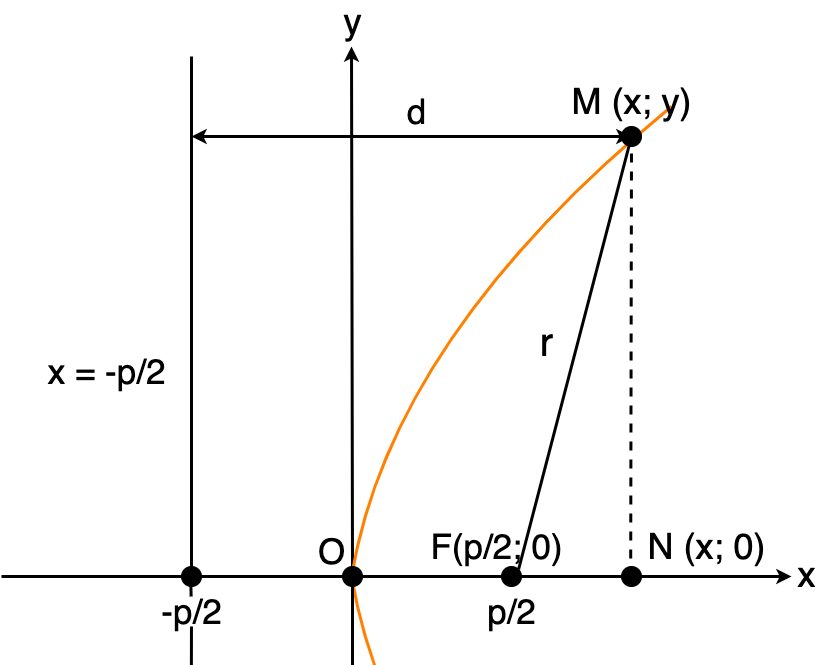
\includegraphics[width=0.8\textwidth]{parabola.png}
\end{center}

Расстояние от т. \(M(x;y)\) до директрисы равно \(d = \Big| x + \dfrac{p}{2} \Big| \).

По определению параболы \(r = d\).

По теореме Пифагора из прямоугольного \(\Delta FMN\): \(r=\sqrt{\Big(x - \dfrac{p}{2}\Big)^2 + y^2}\)

Следовательно:

\begin{gather*}
    \sqrt{\Big(x - \frac{p}{2}\Big)^2 + y^2} = x + \frac{p}{2} \\
    x^2 - px + \frac{p^2}{4} + y^2 = x^2 + px + \frac{p^2}{4} \\
    y^2 = 2px
\end{gather*}

\subsection*{Свойства параболы}

\begin{itemize}
    \item[—]{Имеет ось симметрии называемой осью параболы. Ось проходит через фокус и вершину перпендикулярно директрисе;}
    \item[—]{Если фокус параболы отразить относительно касательной, то его образ будет лежать на директрисе;}
    \item[—]{Все параболы подобны. Расстояние между фокусом и директрисой определяет масштаб;}
\end{itemize}

\end{document}
